\documentclass[t, 				             
			   final,
			   12pt, 				         
			   xcolor={usenames,dvipsnames}, 
			   table]{beamer}

% pacotes utilizados.
\usepackage[alf]{abntex2cite}
\usepackage{amsmath}
\usepackage[brazil]{babel}
\usepackage{booktabs}
\usepackage{caption}
\usepackage[utf8]{inputenc}
\usepackage{listings}
\usepackage{multicol}
\usepackage{multirow}
\usepackage{todo}


% configuração do tema
\usetheme[pageofpages=de,
          bullet=square,			
          titleline=true,				
          alternativetitlepage=true,			
          titlepagelogo=imagens/logo-puc,	
          watermarkheight=70px,		
          watermarkheightmult=4	
          ]{Torino}

\setbeamertemplate{sections/subsections in toc}[square]
\setbeamertemplate{bibliography item}[default]

\usecolortheme{freewilly}

% Block Environment
% -------------------------------
\setbeamertemplate {blocks}[default]
\setbeamercolor{block title}{fg=red!0!green!15!blue!85!, bg=red!33!green!37!blue!15!}
\setbeamercolor{block body}{fg=black, bg=red!32!green!33!blue!5}
\setbeamercolor{block title alerted}{fg=white, bg=red!40!black}
\setbeamercolor{block body alerted}{fg=black, bg=red!5!white}
\setbeamercolor{block title example}{fg=white, bg=green!40!black}
\setbeamercolor{block body example}{fg=black, bg=green!5!white}
\setbeamerfont{block title}{size=\scriptsize, series=\bfseries}


\definecolor{javared}{rgb}{0.6,0,0} % for strings
\definecolor{javagreen}{rgb}{0.25,0.5,0.35} % comments
\definecolor{javapurple}{rgb}{0.5,0,0.35} % keywords
\definecolor{javadocblue}{rgb}{0.25,0.35,0.75} % javadoc
 
\lstset{}

\lstdefinestyle{BashInputBasicStyle}{
	language=bash,
	basicstyle=\normalsize\ttfamily,
	columns=fullflexible,
	tabsize=2,
	showstringspaces=false,
	frame=single,
	inputencoding=utf8,
	rulecolor=\color{gray}
}

\lstdefinestyle{BashInputStyle}{
  language=bash,
  basicstyle=\normalsize\ttfamily,
  numbers=left,
  numberstyle=\tiny,
  numbersep=2pt,
  frame=tb,
  columns=fullflexible,
  tabsize=2,
  showstringspaces=false,
  commentstyle=\color{gray},
  inputencoding=utf8,
  rulecolor=\color{gray}
}

\lstdefinestyle{RubyInputStyle}{
    language=ruby,
    basicstyle=\scriptsize\ttfamily,
    keywordstyle=\color{javapurple},
    identifierstyle=\color{black},
    commentstyle=\color{javagreen},
	stringstyle=\color{blue},
    showstringspaces=false,
    numbers=left,
    numberstyle=\color{gray}\tiny,
    tabsize=3,
    extendedchars=\true,
    inputencoding=utf8,
%   frame=single, 
    columns=fixed,
    backgroundcolor=\color{red!32!green!33!blue!5}
}    
%  language=ruby,
%  basicstyle=\normalsize\ttfamily,
%  keywordstyle=\color{OrangeRed},
%  identifierstyle=\color{Turquoise},
%  commentstyle=\color{gray},
%  stringstyle=\color{YellowOrange},
%  numbers=left,
%  numberstyle=\tiny,
%  numbersep=2pt,
%  frame=tb,
%  columns=fullflexible,
%  backgroundcolor=\color{white!80},
%  linewidth=0.9\linewidth,
%  tabsize=2,
%  showstringspaces=false
%  inputencoding=utf8


\lstdefinestyle{JavaInputStyle}{
	language=Java,
	basicstyle=\ttfamily,
	keywordstyle=\color{javapurple}\bfseries,
	stringstyle=\color{javared},
	commentstyle=\color{javagreen},
	morecomment=[s][\color{javadocblue}]{/**}{*/},
	numbers=left,
	numberstyle=\tiny\color{black},
	numbersep=10pt,
	tabsize=2,
	showspaces=false,
	showstringspaces=false,
	frame=tb,
	columns=fullflexible,
	backgroundcolor=\color{white!80},
	linewidth=0.9\linewidth,
	inputencoding=utf8
}

\begin{document}
    \author{Luiz Alberto Ferreira Gomes}
    \title{Ruby On Rails: Laboratório 01}
    \subtitle{Laboratório de Engenharia de Software}
    \institute{Curso de Ciência da Computação}
    \date{\today}

	\begin{frame}[plain]
  \titlepage
\end{frame}
	\AtBeginSection[]
{
  \begin{frame}{Agenda}
    \tableofcontents[currentsection]
  \end{frame}
}
  	
    
    \section{Ruby on Rails}
	%-------------------------------------------------------------------------------------- Início
\begin{frame}[fragile, plain, c]{Rails}
	\begin{center}
		\large Rails é um \alert{framework} para construção de \alert{aplicações web} baseado na \alert{linguagem Ruby}.
	\end{center}
\end{frame}
%-------------------------------------------------------------------------------------- Início
\begin{frame}[fragile, t]{Rails}
	\begin{itemize}
		\item Uma \alert{gem} (pacote) escrita em Ruby
		\item 100\% \alert{open-source}, MIT License
		\item Fornece \alert{geradores} de código e scripts de \alert{automação} de testes
		\item Ferramentas adicionais são fornecidas no ecossistema Rails:
	\end{itemize}
\end{frame}

%-------------------------------------------------------------------------------------- Início
\begin{frame}[fragile, t]{Ferramentas Adicionais}
	\begin{itemize}
		\item \alert{Rake} - utilitário similar ao \textbf{make do Unix} para criar e migrar bancos de dados, limpar sessões de uma Web app
		\item \alert{Puma} - servidor web de desenvolvimento para execução de aplicações Rails
		\item \alert{SQLite} - um servidor de banco de dados simples pré-instalado como o Rails
		\item \alert{Rack Middleware} - interface padronizado para interação entre um servidor web e uma Web App
	\end{itemize}
\end{frame}	
	%%\section{Histórico de Evolução}
%-------------------------------------------------------------------------------------- Início
\begin{frame}[allowframebreaks,fragile,t]{Histórico do Rails}
  \begin{itemize}
    \item David Hanson \alert{derivou} a partir do BaseCamp da 37Signals
    \item 07/2014 - a primeira versão de código aberto liberada
    \item 02/2015 - direitos \alert{colaboração} com o projeto foram liberados
    \item 08/2006 - Apple distribui no Mac OS X "Leopard"
    \item Rails é utilizado pela companhias Airbnb, Disney, GitHub, Shopify e Twitter.
  \end{itemize}

  \begin{figure}[h]
    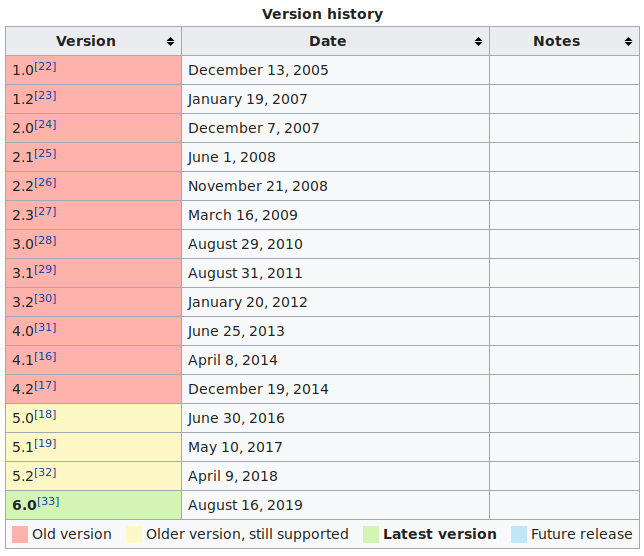
\includegraphics[scale=0.3]{imagens/rails-history.png}  
  \end{figure}
\end{frame}

	\begin{frame}[fragile,t]{Filosofia do Rails}
  \begin{itemize}
    \item Convention Over Configuration (CoC)
    \item Don't Repeat Yourself (DRY)
    \item Representational State Transfer (REST)
  \end{itemize}   
\end{frame}

\begin{frame}[fragile, c]{Convention Over Configuration}
  \begin{center}
    \large se a nomeação \alert{segue} certas \alert{convenções}, não há necessidade de arquivos de \alert{configuração}.
  \end{center}   
\end{frame}

\begin{frame}[fragile, c]{Don't Repeat Yourself}
  \begin{center}
    \large sugere que escrever que o \alert{mesmo código} várias vezes é uma \alert{coisa ruim}
    \end{center}
\end{frame}

\begin{frame}[fragile,t]{Representational State Transfer}
  \begin{center}
    \item organiza a sua aplicação em torno de \alert{recursos} e \alert{padrões} HTTP (verbs)
  \end{center}   
\end{frame}
	%%\section{MVC em Ação no Rails}
%%-------------------------------------------------------------------------------------- Início
\begin{frame}[t, fragile]{Model-View-Controller}
	\begin{itemize}
		\item O framework Rails é contruído em cima do Design Pattern Model View Controller(MVC):
	\end{itemize}
	\begin{figure}[h!]
		\centering
		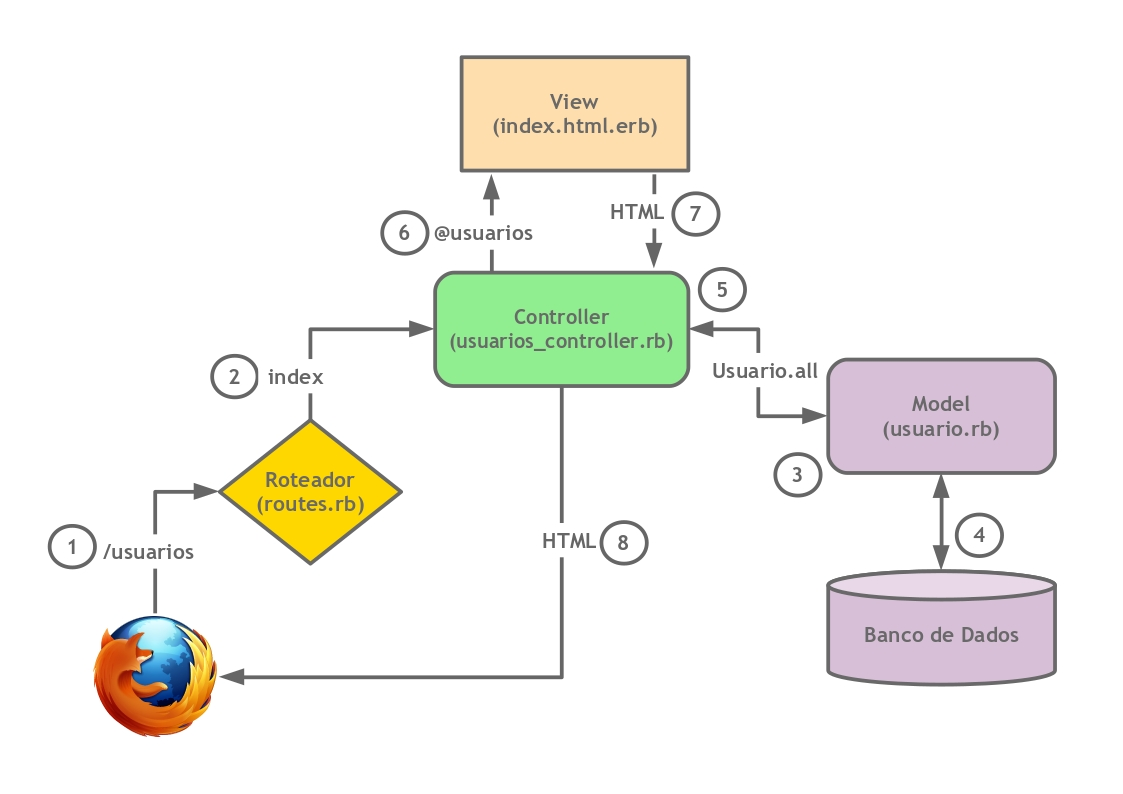
\includegraphics[width=0.70\textwidth]{imagens/mvc.jpg}
	\end{figure}
\end{frame}
 

    
    \section{Metodologia de Trabalho}
    \begin{frame}[fragile,t]{Metodologia de Trabalho}
	\begin{figure}[h!]
		\centering
		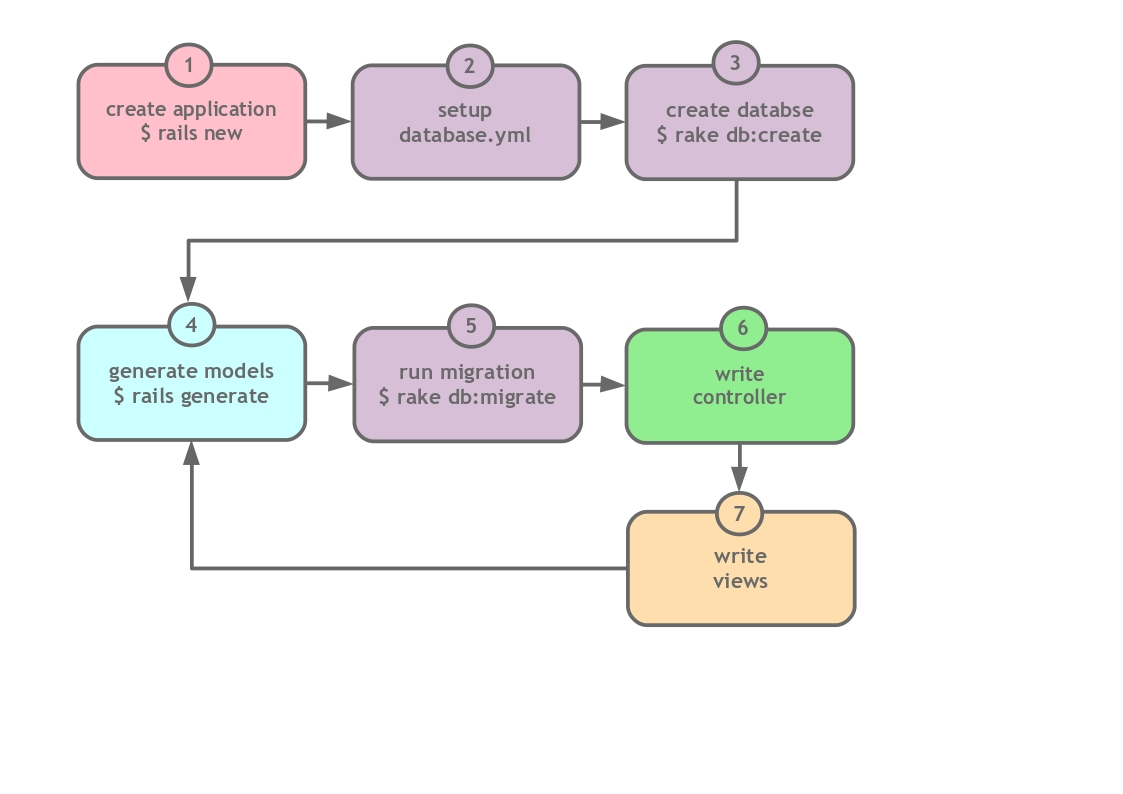
\includegraphics[width=.9\textwidth]{imagens/metodologia-de-trabalho.jpg}
	\end{figure}
\end{frame}


    \section{Esqueleto da Aplicação}
    
\begin{frame}[allowframebreaks,fragile,t]{Estrutura de uma Aplicação Rails}
  \begin{figure}[h]
    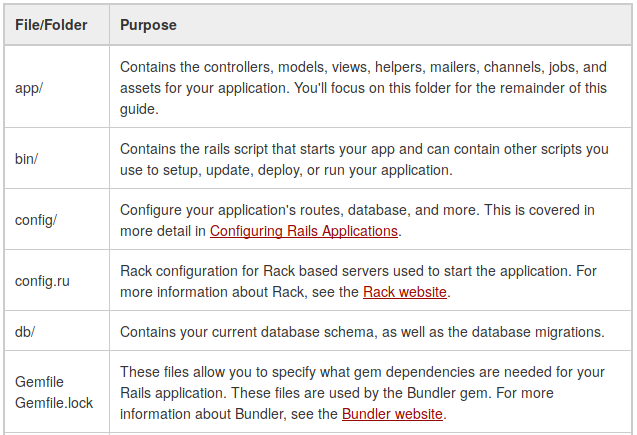
\includegraphics[scale=0.35]{imagens/rails-esqueleto-01.png}  
  \end{figure}
  \begin{figure}[h]
    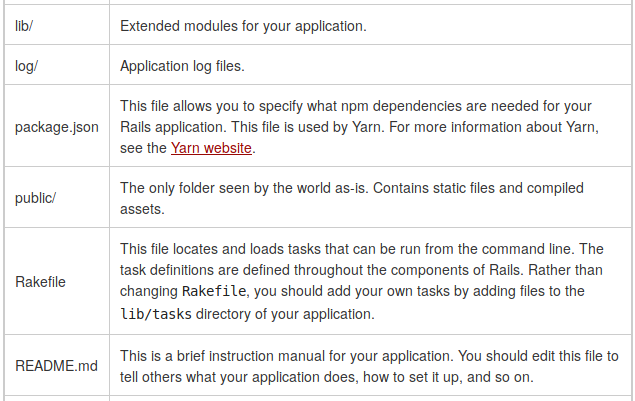
\includegraphics[scale=0.35]{imagens/rails-esqueleto-02.png}  
  \end{figure}
  \begin{figure}[h]
    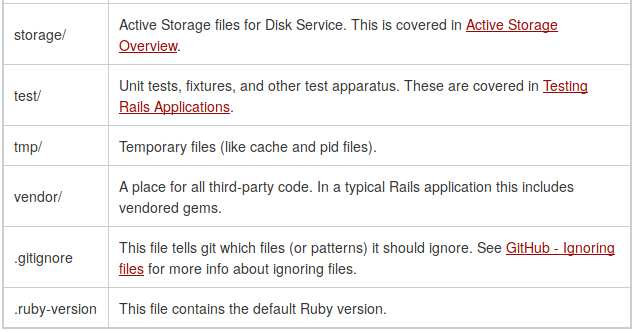
\includegraphics[scale=0.35]{imagens/rails-esqueleto-03.png}  
  \end{figure}
\end{frame}
   
    \section{Pŕatica}
    
\begin{frame}[fragile,t]{Prática de Laboratório (Para Casa)}
  \begin{itemize}
      \item Instale no seu computador ou configure o ambiente Plaza Cloud para as 
      próximas práticas de laboratório.
  \end{itemize}
\end{frame}

    \section{Para Saber Mais}
    %%-------------------------------------------------------------------------------------- Início
\begin{frame}[fragile,t]{Para Saber Mais}
  \begin{itemize}
    \item \url{https://www.ruby-lang.org/en/}
    \begin{itemize}
     \item referência oficial da linguagem Ruby onde a toda a sua documentação está disponível
	para ser consultada.
    \end{itemize}

    \item \url{http://rubyonrails.org/}
    \begin{itemize}
     \item referência oficial do framework Rails onde a toda a sua documentação está disponível
	para ser consultada.
    \end{itemize}
    
    \item \url{http://www.codecademy.com/pt/tracks/ruby}
    \begin{itemize}
     \item curso iterativo em portugês sobre a linguagem Ruby.
    \end{itemize}

	\item \url{https://gorails.com/setup/ubuntu/16.04}
	\begin{itemize}
		\item guia para instalação do Ruby on Rails no Ubuntu e no Mac OSX.
	\end{itemize}
  \end{itemize}
  
  
\end{frame}
\end{document}
